\documentclass[11pt,a4paper]{article}
\usepackage[utf8]{inputenc}
\usepackage[german]{babel}
\usepackage{amsmath}
\usepackage{amsfonts}
\usepackage{subfig}
\usepackage{amssymb}
\usepackage{siunitx,physics}
\usepackage{mathtools}
\usepackage{graphicx}
%\usepackage{Here}
\usepackage[version=4]{mhchem}
\usepackage{url}
\usepackage{setspace}
\usepackage[left=2.5cm,right=2.5cm,top=2.5cm,bottom=2cm]{geometry}
[biblography=totocnumbered]
\usepackage{fancyhdr}
\usepackage{scrextend}
\usepackage{hyperref}
\pagenumbering{gobble}

\makeatletter
\newcommand\bigcdot{\mathpalette\bigcdot@{.5}}
\newcommand\bigcdot@[2]{\mathbin{\vcenter{\hbox{\scalebox{#2}{$\m@th#1\bullet$}}}}}
\makeatother

\makeatletter
%\renewcommand*\bib@heading{%
%  \subsection*{}%
%  \@mkboth{\refname}{\refname}}
%\makeatother
\numberwithin{equation}{section}
\numberwithin{figure}{section}

\renewcommand{\labelitemii}{\labelitemfont$\vartriangleright$}
\begin{document}\\
\begin{addmargin}[25pt]{0pt}
In Keramiken mit einer regelmäßigen Anordnung von Kationen und Anionen kann entweder ein Kation oder ein Anion fehlen oder es können auch 2 Kationen den gleichen Zwischengitterplatz einnehmen, siehe Abbildung \ref{fig:Fehlstellen_Keramiken}. Ein Anion auf einem Zwischengitterplatz ist sehr unwahrscheinlich da Anionen sehr viel größer sind als Kationen. Diese beschriebenen Gitterdefekte können jedoch nicht einzeln auftreten, da in Keramiken die Elektroneutralität eingehalten werden muss. Deswegen gibt es in der Realität immer entweder einen Schottky-Defekt, also eine Kombination aus Anion- und Kationfehlstelle oder einen Frenkel-Defekt, das ist eine Kombination aus Kationfehlstelle und einem zusätzlichen Zwischengitterkation.\\
\begin{figure}[h]
    \centering
    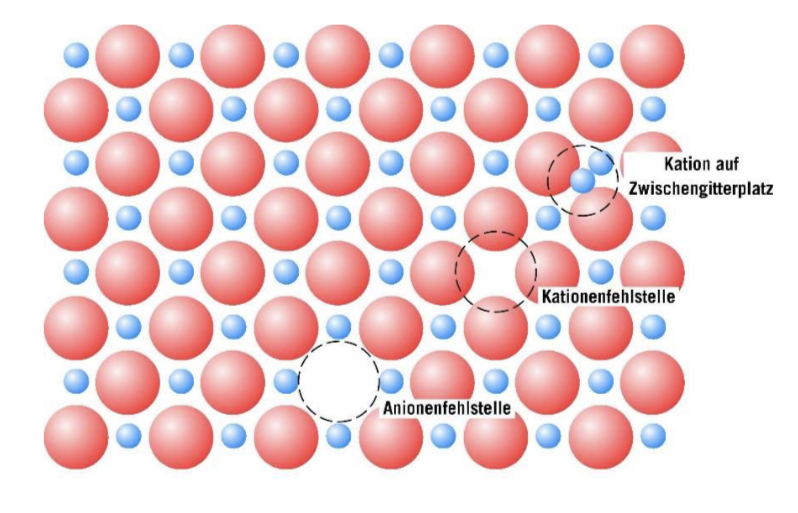
\includegraphics[width = 0.8\textwidth]{images/Materialwissenschaften/Fehlstellen_Keramiken.jpeg}
    \caption{Die verschiedenen Arten von Fehlstellen in Keramiken}
    \label{fig:Fehlstellen_Keramiken}
\end{figure}
\end{addmargin}

\end{document}